\documentclass[11pt,a4paper,twoside]{article}
%%%%%%%%%%%%%%
\usepackage{etoolbox}  % used in jmpag.sty
\usepackage{forloop}    % used in jmpag.sty
%%%%%%%%%%%%%%
\usepackage{amsthm,amsfonts,amsmath,amscd,amssymb}
\usepackage{latexsym}
\usepackage{euscript}
\usepackage{enumitem}
%\usepackage{rotating}
\usepackage{graphicx}
%\usepackage{epstopdf}
\usepackage{tikz}
\usepackage{caption}
\usepackage{subcaption}
\usepackage{cite}
\usepackage[utf8]{inputenc}
\usepackage[english]{babel}
\usepackage{xcolor}
\usepackage{multirow}
\definecolor{darkgreen}{HTML}{00A000}
\definecolor{darkblue}{HTML}{0000A0}
\definecolor{darkred}{HTML}{D00000}
\usepackage[colorlinks=true]{hyperref}%%%%%%%%%[,backref]!!!!!!!!!!!!!!!!!!!!
\hypersetup{linkcolor=darkred, urlcolor=darkblue, citecolor=darkgreen}%%%%%%%%
%
%%%%%%%%%%%%%%%%%%%%%% YOUR PACKAGES %%%%%%%%%%%%%%%%%%%%%%%%%%%%%%


%%%%%%%%%%%%%%%%%%%%%% END YOUR PACKAGES %%%%%%%%%%%%%%%%%%%%%%%%%%

\usepackage{jmpag}

%%%%%%%%%%%%%%%%%%%%%%%%%%%%%%%%%%%%%%%%%%%%%%%%%%
\tolerance=9000
\textwidth=135mm%11pt
\textheight=216.5mm %196.5mm%11pt
\oddsidemargin=0mm
\evensidemargin=25mm
\topmargin-10mm

\pagestyle{jmpag}

%%%%%%%%%%%%%%%%%%%%%%%%%%%%%%%%%%%%%%%%%%%%%%%%%%%%%%%%%%%%%%

%%%%%%%%%%%%%%%%%%%%%%%%%%%%%%%%%%%%%%%%%%%%%%%%%%%%%%%%%%%%%%%%

\begin{document}

%%%%%%%%%%%%%% TITLE and AUTHORS %%%%%%%%%%%%%%%%%%

% The full title of your paper
\title{Numerical Study of Soliton Solutions to the Two Dimensional Boussinesq  Equation}

% If the title of your paper is too long, use the short title please. It should not exceed 60 symbols (including blank spaces).

%\title[Short Title]{Title}


% Author1
%FirstName1 LastName1
\author{Krassimir Angelow}
%Institution1, address1, City1, Postal Code1, Country
\address{Bulgarian Academy of Sciences, Institute of Mathematics and Informatics, ul. Acad. G. Bonchev, block 8, 1113 Sofia, Bulgaria}
%e-mail1
\email{angelow@math.bas.bg}

% Author2
%FirstName2 LastName2
\author{Natalia Kolkovska}
%Institution2, address2, City2, Postal Code2, Country2
\address{Bulgarian Academy of Sciences, Institute of Mathematics and Informatics, ul. Acad. G. Bonchev, block 8, 1113 Sofia, Bulgaria}
%e-mail2
\email{n.kolkovska@gmail.com}


%%%%%%%%%%%%%%%% END TITLE and AUTHORS %%%%%%%%%%%%%%%%%%%

\BeginPaper %%%%%%% do not remove this command

%%%%%%%%%%%%%%%%%%%%%% MY MACROS %%%%%%%%%%%%%%%%%%%%

\newcommand{\ep}{\varepsilon}
\newcommand{\eps}[1]{{#1}_{\varepsilon}}
\newcommand{\rf}[1]{(\ref{#1})}
\newcommand{\RR}{\mathbb{R}}

%%%%%%%%%%%%%%%%%%%%% END MY MACROS %%%%%%%%%%%%%%%%%%%%%%

%%%%%%%%%%%%%%%%%%%%%%% ABSTRACT %%%%%%%%%%%%%%%%%%%%%%%%

\begin{abstract}
This paper evaluates propagating wave solutions to the two dimensional Boussinesq Equation (BE). To solve this nonlinear fourth order hyperbolic problem we use Fast Poisson Solver with high order finite difference schemes for the spatial derivatives. Taylor Series (TS) expansion about time is used to move the soliton forward. A Boundary Condition (BC) is applied on the computational boundary. The performed numerical tests exhibit good convergence and confirm the validity of the TS method.



\key{differential equation, two dimensional Boussinesq equation, traveling wave solutions (TWS), high order finite difference schemes, Fast Poisson Solvers.}

\msc{34L15, 34L20, 35R10}
\end{abstract}


%%%%%%%%%%%%%%%%%%%% END ABSTRACT %%%%%%%%%%%%%%%%%%%%%%%%%%%%%

%The title of your section
\section{Introduction.}\label{introduction}

In this paper we  consider the two dimensional Boussinesq  Equation (BE)
\begin{align} \label{eq1}
&u_{tt} - \Delta u -\beta_1  \Delta u_{tt} +\beta_2 \Delta ^2 u + \Delta f(u)=0   \quad \text{for}  (x,y) \in \RR^2, \, t\in\RR^+, 
\\ \nonumber &u(x,y,0)=u_0(x,y), \, u_t(x,y,0)=u_1(x,y)   \quad\text{for} \, (x,y) \in \RR^2,
\\  &u(x,y) \rightarrow 0,  \Delta u(x,y) \rightarrow 0 ,  \quad \text{for}  \sqrt{x^2 + y^2} \rightarrow \infty, \label{eq11}
\end{align}
where $f(u)=\alpha u^2$,  $\alpha>0$, $\beta_1>0$, $\beta_2>0$  are dispersion parameters, and $\Delta$ is the Laplace operator. The BE is famous with the approximation of shallow water waves or also weakly non--linear long waves. It is often used for simulation of various physical processes e.g. turbulence in fluid mechanics, vibrations in acoustics, geotechnical engineering, athmosphere dynamics etc. A derivation of the BE from the original Boussinesq system can be found in \cite{ChChr}. In order to obtain an initial condition (IC) for equation \rf{eq1}, \rf{eq11}, it is required to solve another elliptic differential equation with similar terms. An approximation for IC with small wave velocities $c$ was developed in \cite{Ch2011}. Other methods for obtaining IC were developed in \cite{chr-chr},\cite{chr-chr-07} and \cite{EllipticProblem}. The asymptotic of the solution function is also an important topic and was mainly researched in \cite{chr-chr-07}, \cite{Ch2012} and \cite{BoundaryProblem}. If the aymptotic behavior is known, then one could use a finite domain $\Omega$ with $u:\Omega \rightarrow \RR$ and apply the corresponding boundary conditions on $\partial \Omega$. Let us once again recall the initial equation \rf{eq1}, \rf{eq11}. The articles \cite{cher} and \cite{dani} showed results for the hyperbolic problem \rf{eq1} with small wave speeds $c \approx 0.3$ and used the Perturbation Solution, which is developed in \cite{Ch2011}, as IC . There, the wave either blows up or vanishes very quickly. Thus, the following article appeared \cite{critEn}, which gives the partial answer whether the IC is going to blow-up, depending on the computation of the critical energy constant for the two-dimensional BE. Nevertheless, there are still no tests in the literature for \rf{eq1} with higher wave speeds $c \approx min(1, 1/\sqrt{\beta_1})$ and no tests with IC different from the Perturbation Solution in \cite{Ch2011}. The last seems to be very adaptive and useful as the author gives an explicit formula in two dimensions. Unfortunately, the formula has its limitations and downsides. 
The obtained results in our previous work \cite{EllipticProblem} and \cite{BoundaryProblem} serve as initial and boundary condition for the hyperbolic equation \rf{eq1}, \rf{eq11}  here. In order to relate to \cite{EllipticProblem} and \cite{BoundaryProblem}
the following variable change is applied
\begin{equation}\label{vc}
x = \sqrt{\beta_1} \tilde x, \quad y = \sqrt{\beta_1} \tilde y, \quad t = \sqrt{\beta_1} \tilde t, \quad \tilde \Delta = \tilde u_{\tilde x \tilde x} + \tilde u_{\tilde y \tilde y}
\end{equation}
which transforms the main equation \rf{eq1}  into 
\begin{equation}\label{eqVC}
(E-\tilde \Delta)  \tilde u_{\tilde t \tilde t} = \frac{(E-\tilde\Delta)\tilde\Delta \tilde u + \alpha \beta \tilde\Delta(\tilde u^2) + (\beta -1)\tilde\Delta \tilde u}{\beta},
\end{equation}
where $\beta = \beta_1 / \beta_2$. The goal of the article is to seek for soliton solutions to \rf{eqVC}, which 
are traveling  in $y$ direction with velocity $c$. TS expansion is used to calculate the next time layer with respect to the time step $\tau$. The time derivatives
are obtained from the equation \rf{eqVC} by an iterative procedure. This is possible because the equation allows to isolate the highest time derivative on one side of the equation. By differentiating with respect to time variable one could obtain higher time derivative terms in the TS expansion. Here, the solver could be adjusted to use second, fourth or sixth approximation order, i.e. $O(\tau^2)$, $O(\tau^4)$, $O(\tau^6)$. To increase the precision of the numerical method, finite difference schemes (FDS) with local approximation of forth $O(h^4)$ and sixth $O(h^6)$ order are applied to the spatial derivatives i.e.  second derivatives along space are approximated with high order finite differences. Thus, the numerical solution is computed on relatively coarse grid with high accuracy. The inversion of $(E - \tilde \Delta)$ operator is discussed in section \rf{FPSsection}. Using spectral analysis, one could decompose the discrete version of the operator by finding its eigenvectors and corresponding eigenvalues. After a suitable substitution $n$ linear systems $A_{i,i} \bar u_i = \bar f_i$, $i = 1,...,n$ are obtained where $n$ is the discrete step count along the $x$ axis. The best part is that the matrices $A_{i,i}$ are tri-, five-, or seven-diagonal depending on the local approximation used for the second derivatives in the discrete laplace operator, i.e. second $O(h^2)$,  fourth $O(h^4)$ or sixth $O(h^6)$ respectively. In order to compare the results from TS method, a conservative finite difference scheme with weights is used, which applies second order of approximation along time and space.
Both methods are tested with zero boundary and also with BC found and developed in \cite{BoundaryProblem}.

\section{Taylor Series Approach for the BE in Two Dimensions}\label{TaylorA}

Revert to old abbreviations $x$, $y$, $t$ and $u$ and define $L$ to be an operator of the form
\begin{equation}\label{operator}
Lu = \frac{\Delta u + (E-\Delta)^{-1} ( \alpha \beta \Delta( u^2) + (\beta -1)\Delta u)}{\beta},
\end{equation}
where the negative power denotes the inverse operator of $(E-\Delta)$. The finite differences along time and space require TS expansions of $u(x,y,t)$. Therefore it is assumed that the solution is $s$ times infinitely differentiable with respect to $t$ and $p$ times infinitely differentiable with respect to $x$ and $y$, i.e. $u \in C^s(T, R)$ and $u \in C^p(\Omega, R)$. For simplicity $s$ also stands for the order of the TS expansion and $p$ stands for the order of the FDS approximations along the computational box $\Omega_h$. It is shown that the error of the method is $O(h^p + \tau^s)$ if a suitable boundary condition is applied on $\partial \Omega_h$.

If the two dimensional differential operator $(E-\Delta)$ is discretized numerically by finite differences then it can be inverted using Fast Poisson Solvers \cite{FPS}. The last algorithm produces band matrices which need to be inverted. Thomas algorithm is used for three diagonal matrices and $O(h^2)$ approximation order.  Five and seven diagonal matrices (with $O(h^4)$ and $O(h^6)$ approximation order, respectively) use similar to Thomas technique which is again a simplified form of Gauss elimination.

The solution function $u$ is defined by $u : \bar \Omega \times T \rightarrow  R$ where $\bar \Omega = \partial \Omega \cup \Omega$. If $\Omega_h$ is the corresponding grid to $\bar \Omega$ with equal step size $h$ along $x$ and $y$ directions, then $u_h$ is defined as the restriction of $u$ over $\Omega_h$
$$u_h : \bar \Omega_h \times T \rightarrow  R$$
$$ (x,y) \in \bar \Omega_h \rightarrow u_h(x,y, t_k)$$
for arbitrary $t_k \in T$. The spatial derivatives discretization in \rf{eqVC} is made by using centered finite differences and extending the stencil:
\begin{equation}\label{fd}
u_{\widehat{xx},p}(x) :=  \frac{1}{h^2} \sum\limits_{i=-p/2}^{p/2} d_i u(x+ih),
\end{equation}
 Here $p$ is equal to $2$, $4$ or $6$.  The weights $d_i$ which are taken from \cite{forn} are  
 $ 1,-2,1$ for $p=2$, $-\frac{1}{12}, \frac{4}{3}, -\frac{5}{2}, \frac{4}{3}, -\frac{1}{12}$ for $p=4$ and  $\frac{1}{90}, -\frac{3}{20}, \frac{3}{2}, -\frac{49}{18}, \frac{3}{2}, -\frac{3}{20}, \frac{1}{90}$ for $p=6$. The approximation error of  formulae \rf{fd} is $O(h^p)$. Replacing the Laplace operator in \rf{eqVC} by the discrete Laplacian 
$$ \Delta_{h,p} v_{i,j} := (v_{i,j})_{\widehat{xx},p} + (v_{i,j})_{\widehat{yy},p}$$ 
we obtain finite difference schemes with high order of approximation $O(h^4)$ for $p=4$ and  $O(h^6)$ for $p=6 $.  The application of FDS with high order of approximation leads to a high rate of convergence of the method for sufficiently smooth solutions. In this way more accurate solutions can be produced on a coarse grid. An explicit formula for the highest derivative of $u$ in PDE \rf{eqVC} 

\begin{equation}\label{Leq}
\frac{ \partial^2 u_h }{ \partial t^2 } = L_h u_h = \frac{ \Delta_h u_h + (E - \Delta_h)^{-1} ( \alpha \beta \Delta_h( u_h^2) + (\beta -1)\Delta_h u_h) }{\beta}
\end{equation}
is obtained. The solution is $s$ times differentiable on $T$ and therefore the last transforms into

\begin{equation}\label{DLeq}
D^{\tilde s} (u_h) =\frac{ \Delta_h D^{\tilde s - 2}(u_h) + (E - \Delta_h)^{-1}( \Delta_h D^{\tilde s - 2} ( \alpha \beta u_h^2  + (\beta -1)u_h) )  }{\beta} 
\end{equation}

with $D^{(\tilde s)} := \partial^{\tilde s} / \partial t^{\tilde s}$ and $\tilde s = 2,...,s$. The $\tilde s^{th}$ time derivative requires $(\tilde s-2)^{th}$, $(\tilde s-3)^{th}$, ..., $2^{nd}$ and $1^{st}$ derivatives and the function $u_h$ itself. E.g. if one would like to calculate the $7^{th}$ derivative $\partial^7 u / \partial t^7$, then $5^{th}$, $4^{th}$, $3^{rd}$, $2^{nd}$, $1^{st}$ and $0^{th}$ derivatives are used and the $5^{th}$ requires  $3^{rd}$, $2^{nd}$, $1^{st}$ and $0^{th}$ and so on.  Thus if $\psi$ and $\bar \psi$ are two known functions with $\psi(x,y) = u(x,y, t_k)$ and $\bar \psi(x,y) = u_t(x,y, t_k)$ then the derivative $\partial^{\tilde s} u / \partial t^{\tilde s}$ could be expressed solely by $\psi$ and $\bar \psi$ at $t = t_k$.

%=============BEGIN Formal Def========================================
\iffalse
Formal (Long) version:
Let's define the following function set
\begin{equation}
Q_{\tilde s}(u_h) := \{ D^{q}(u_h), q = 0, ... , \tilde s - 2 \}.
\end{equation}
In order to describe the iterative process in short notations the following vector valued functions are defined
\begin{align*} 
P_{\tilde s} : \Omega_h^{(\tilde s - 1)} \rightarrow \Omega_h
\\ Q_{\tilde s}(u_h(t_k)) \rightarrow P_{\tilde s} (Q_{\tilde s}(u_h) ) = L_h( D^{(\tilde s - 2)} (u_h(t_k)) ).
\end{align*}

Example 1. The PDE \rf{eqVC} can be expressed through 
\begin{equation}\label{example}
D^{2}(u_h) = P_0(Q_0(u)) + O(h^p) = P_0(u_h) + O(h^p),
\end{equation}
which is equation \rf{Leq} written in short form. When the operator $D^{(\tilde s -2)}$ is applied on both sides of equation \rf{example}, it follows that
\begin{equation}\label{DPeq}
D^{\tilde s}(u_h) = P_{\tilde s}(Q_{\tilde s}(u)) + O(h^p))
\end{equation}
which is the short form of \rf{DLeq}. Now let $\tilde s = 6$, then \rf{DPeq} reads as

\begin{align*} 
D^6 u_h - O(h^p) = P_4(Q_4(u_h)) =
\\
= P_4(\{u_{ h}, u_{ h_{t} }, u_{ h_{tt} }, u_{ h_{ttt} }, u_{ h_{tttt} } \}) = 
\\
= P_4(\{u_{ h}, u_{ h_{t} }, P_0(\{u_h\}),  P_1( \{ u_h, u_{ h_{t} } \} ), P_2( \{ u_h, u_{ h_{t} }, u_{ h_{tt} } \} )  \}) = 
\\ 
= P_4(\{u_{ h}, u_{ h_{t} }, P_0(\{u_h\}),  P_1( \{ u_h, u_{ h_{t} } \} ), P_2( \{ u_h, u_{ h_{t} },  P_0( \{ u_h \} ) \} )  \}).
\end{align*}

Example 2. Let's look at PDE \rf{eqVC}. For $\tilde s = 2$:
$$
u_{tt} = Lu.
$$
For $\tilde s = 3$:
$$
u_{ttt} = L(D(u)) = \frac{ \Delta u_t + (E - \Delta)^{-1}           ( \Delta (2 \alpha \beta u u_t  +                          (\beta -1)u_t) )  }{\beta}.
$$
For $\tilde s = 4$:
$$
u_{tttt} = L(D^2(u)) = \frac{ \Delta u_{tt} + (E - \Delta)^{-1}( \Delta (2 \alpha \beta ( u Lu +  u_t^2 )   + (\beta -1) u_{tt} ) )  }{\beta}.
$$

A more general formula, which is relevant only to the complexity of the algorithm, i.e. to estimate the number of operations for its calculation, is

\begin{align*}
\beta LD^{(\tilde s)} u =   \Delta D^{ (\tilde s - 2) }(u)  +
\\
 (E - \Delta)^{-1}( \Delta ( \alpha \beta \sum_{j=0}^{ \tilde s - 2}  { \tilde s - 2\choose j} D^j(u) D^{ (\tilde s - 2 - j) }(u)+ (\beta -1) D^{ (\tilde s - 2) }(u) ) ).
\end{align*}
Nevertheless the formula itself is not our goal, just use the computer to derive it and evaluate it for a given function set $Q_{\tilde s}$.
\fi

%=============END Formal Def========================================

Till now only space discretization, with step $h$, is applied on $\Omega$ and equation \rf{DLeq}. First, Let's define $t_k = \tau k$, $k \in N \cup \{0\}$, where $\tau$ is the time step and $t_k \in T_{\tau}$ describes the time domain. Second, let's take an IC $u_0(x,y) = u(x,y,0)$ and $u_1(x,y) = u_t(x,y,0)$ from \cite{EllipticProblem}. Third, 
a polynomial of second degree around $t_k$ approximates $u_h$
\begin{equation}\label{taylor21}
u_h(t_{k+1}) = u_h(t_k+\tau) = u_h(t_k) + \frac{\tau } {1!} \frac{ \partial }{ \partial t } u_h( t_k ) + \frac{ \tau^2 } { 2! }L_h u_h( t_k ) + O(\tau^3)
\end{equation}
and a polynomial of first degree around $t_k$ approximates $u_{h_t}$

\begin{equation}\label{taylor22}
\frac{ \partial } { \partial t } u_h( t_{k+1} ) = \frac{\partial } { \partial t }u_h(t_k) + \frac{\tau } {1!} L_h u_h(t_k) + O(\tau^2),
\end{equation}
where we use equality \rf{Leq} in the last term of the TS. Then, the formulae \rf{taylor21} and \rf{taylor22} define an iterative procedure with second approximation order along time, and the IC $u_0(x,y) = u_h(0), u_{1_h}(x,y) = \partial / \partial t (u_h(0))$ is used at the start $t_0 = 0$.

The algorithm could be generalized to use higher terms it the TS expansion. All derivatives $D^{\tilde s}(u(t_k))$ could be found iteratively for each $2 \leq \tilde s \leq s$ through \rf{DLeq}. If the finite difference discretizations applied along space $(E - \Delta_h)^{-1}$ and $\Delta_h$ have order of approximation $O(h^p)$ then Taylor formula gives the following
\begin{align} \label{GeneralIt}
u(x,y,t_{k+1}) = u_h(t_k) + \frac{\tau } {1!}  \frac{\partial}{\partial t} u_h(t_k) + \frac{ \tau^2} { 2!}L_h u_h(t_k) +... + \nonumber
\\ + \frac{\tau^s}{ s! }L_h \frac{\partial^{s-2}}{\partial t^{s-2}} u_h(t_k) + O(h^p + \tau^{s+1}) = u_h(t_{k+1}) + O(h^p + \tau^{s+1}), \nonumber
\\  \frac{\partial}{\partial t}u(x,y,t_{k+1}) = \frac{\partial}{\partial t} u_h(t_k) + \frac{\tau } {1!}  L_h u_h(t_k) + ... + \nonumber
\\ + \frac{\tau^{s-1}}{ (s-1)! } L_h \frac{\partial^{s-2} }{\partial t^{s-2}} u_h(t_k)  + O(h^p + \tau^s) = \frac{\partial}{\partial t}u_h(t_{k+1}) + O(h^p + \tau^s)
\end{align}

Formulae \rf{GeneralIt} define an iterative procedure with approximation order $O(h^p + \tau^s)$ which is easily proved by induction. At each step this numerical procedure calculates TS expansions of two numerical values: $u_h$ and its first derivative $D(u_h)$, because the PDE is of second order in time. 

%=============BEGIN Boundary========================================
\section{Boundary Condition}\label{BndS}
%=============BEGIN Boundary========================================
The following boundary function
\begin{equation}\label{eqBCV}
\widehat U_B(x , y) = \mu_u \frac{ (1 - \tilde c^2/\beta) x^2 - \tilde y^2}{( (1 - \tilde c^2/\beta) \tilde x^2 + \tilde y^2)^2}
\end{equation}
found in \cite{BoundaryProblem} is used to to evaluate stationary propagating wave solutions described in \cite{EllipticProblem}. The last article focus on solutions to \rf{eqVC} of the type $u(x, y, t) = U(x, y - ct)$, which are stationary solitary waves traveling in y direction
with velocity c. In order to use \rf{eqBCV} as BC for \rf{eqVC}, it is transformed into
\begin{equation}\label{eqBCH}
\bar U_B(x_b , y_b, t_b) = \mu_u \frac{ (1 - c^2) x_b^2 - (y_b-ct_b)^2}{( (1 - c^2) x_b^2 + (y_b-ct_b)^2)^2}
\end{equation}
with $c = \tilde c / \sqrt{\beta}$, $x_b = \tilde x$ and $y_b - ct_b = \tilde y$. 
Near the computational boundaries $(x,y):x=L_x$ and $(x,y):y=L_y$ we do not change the stencil \rf{fd}. The discrete Laplacian
is defined there by using the values of the discrete solution \rf{eqBCH} at points outside the computational domain. The value of $\mu_u$ is obtained again from the method developed in \cite{BoundaryProblem}. If the second derivative $\partial^2 / \partial x^2$ is approximated with three points, i.e. $p=2$ (green color), then it uses one point outside the computational domain $\Omega_h$. For $p=4$, the derivative $\partial^2 / \partial x^2$ implies five point stencil (blue color) with maximum

\begin{figure}[ht]% It requires \usepackage{graphicx}
\begin{center}
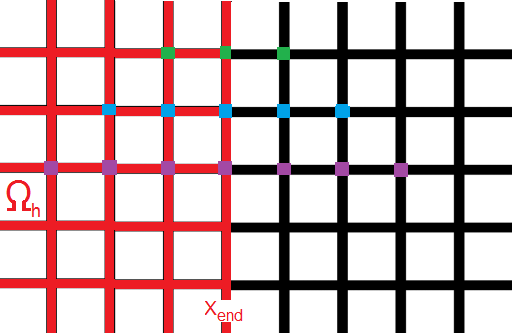
\includegraphics[width=2in]{Pictures/BoundaryPicture.png}
	\caption{Finite Differences near the computational boundary.}
	\label{fig:BoundaryFD}
  \end{center}
\end{figure}
two extra points and for $p=6$, it implies seven point stencil (purple color) with maximum three extra points outside the computational domain $\Omega_h$ (see Figure \ref{fig:BoundaryFD}). Same reasoning is implied for the $\partial^2 / \partial y^2$ derivative. This is a standard procedure which involves symbolic calculation of the following terms:
\begin{align}
& \frac{ \partial^{\tilde s} } { \partial t^{\tilde s} } \widehat U_{B_h}(t_k)
\\
& \alpha \beta \frac{ \partial^{\tilde s} } { \partial t^{\tilde s} } \widehat U_{B_h}(t_k)^2  + (\beta -1)\frac{ \partial^{\tilde s} } { \partial t^{\tilde s} }\widehat U_{B_h}(t_k), \label{nonLinBnd}
\\
& (\beta \frac{ \partial^2 } { \partial t^2 } - \Delta)\frac{ \partial^{\tilde s} } { \partial t^{\tilde s} } \widehat U_{B_h}(t_k) \quad \tilde s = 0,...,s-2 \label{psnBnd}
\end{align}
defined over the "black net" on Figure \ref{fig:BoundaryFD}, i.e. a few points outside the domain $\Omega_h$. The function \rf{nonLinBnd} is used when the $\Delta_h$ operator is applied on the non-linear term and \rf{psnBnd} is used when inverting the $E - \Delta_h$ (see section \rf{FPSsection}).
\iffalse

===========================================================
 The affected terms in equation \rf{Leq} which make use of the boundary function \rf{eqBCV} are the following:
\begin{equation*}
\frac{ \Delta_h u_h}{\beta}, \frac{ (E - \Delta_h)^{-1} ( (\beta -1)\Delta_h u_h) }{\beta}
\end{equation*}
The TS approach also requires time derivatives of both terms defined above
\begin{equation*}
\frac{ \Delta_h D^{(\tilde s)} (u_h)}{\beta}, \frac{ (E - \Delta_h)^{-1} ( (\beta -1)\Delta_h D^{(\tilde s)}(u_h) ) }{\beta}
\end{equation*}
for $\tilde s = 0, ..., s-2$.  Thus, $D^{\tilde s}(\bar U_B(x_b , y_b, t_b))$  time derivative values outside the computational boundary $\partial \Omega_h$ are also used to extend the $p+1$ point stencil where needed (see Figure  \ref{fig:BoundaryFD}). 

As it is noticed in the previous section, the operator $(E - \Delta_h)^{-1}$ does not fully apply on the computational boundary $\partial \Omega_h$. In the previous section, it is defined that

++++++++++++++++++++++++++++++++++++++++++++++++++++++++++++

\begin{equation}
(E-\Delta_h -\Delta_{ext})(\beta \frac{ \partial^2 } { \partial t^2 } - \Delta) u =( \Delta_h + \Delta_{ext}) ( \alpha \beta u^2  + (\beta -1)u) 
\end{equation}

\begin{align}
&(E-\Delta_h)(\beta \frac{ \partial^2 } { \partial t^2 } - \Delta_h - \Delta_{ext}) u_h(t_k) - \Delta_{ext}((\beta \frac{ \partial^2 } { \partial t^2 } - \Delta)\bar U_B(t_k))_h = 
\\
&\Delta_h ( \alpha \beta u_h(t_k)^2  + (\beta -1)u_h(t_k)) +  \Delta_{ext} ( \alpha \beta\widehat U_{B_h}(t_k)^2  + (\beta -1)\widehat U_{B_h}(t_k))  
\end{align}

\begin{align}
&(\beta \frac{ \partial^2 } { \partial t^2 } - \Delta_h - \Delta_{ext}) u_h(t_k)  = 
\\
&(E-\Delta_h)^{-1} ( \Delta_h ( \alpha \beta u_h(t_k)^2  + (\beta -1)u_h(t_k)) +  \Delta_{ext} ( \alpha \beta\widehat U_{B_h}(t_k)^2  + (\beta -1)\widehat U_{B_h}(t_k))   \nonumber
\\
&\Delta_{ext}((\beta \frac{ \partial^2 } { \partial t^2 } - \Delta)\bar U_B(t_k))_h )
\end{align}

\begin{align}
&(\beta \frac{ \partial^2 } { \partial t^2 } - \Delta_h - \Delta_{ext}) u_h(t_k)  = 
\\
&(E-\Delta_h)^{-1} ( \Delta_h ( \alpha \beta u_h(t_k)^2  + (\beta -1)u_h(t_k)) +  \Delta_{ext} ( (\beta -1)\widehat U_{B_h}(t_k))  )
\end{align}
++++++++++++++++++++++++++++++++++++++++++++++++++++++++++++

In order to balance for the incompleteness of $A_h = (E-\Delta_h)$ operator, the following term needs to be subtracted from the right side $f_h$:
\begin{equation*}
(E-\Delta)_{ext}(\beta \frac{ \partial^2 } { \partial t^2 } - \Delta) \widehat U_{B_h}
\end{equation*}
where $(E-\Delta)_{ext}$ is defined only on the "black points" over an extended domain that steps out $\partial \Omega_h$ (see Figure \ref{fig:BoundaryFD}). The identity operator $E$ influences only inside $\bar \Omega_h$ thus the term transforms into
\begin{equation*}
-\Delta_{ext}(\beta \frac{ \partial^2 } { \partial t^2 } - \Delta) \widehat U_{B_h}.
\end{equation*}
which is smaller enough to be neglected.
================================================
\fi
%=============BEGIN FPP========================================
\section{Fast Poisson Solvers and Invertion of $(E-\tilde \Delta)$ in \rf{eqVC}}\label{FPSsection}
%=============BEGIN FPP========================================
Suppose the following linear equaion
\begin{equation}\label{FPeq}
Az:=z-\Delta z = f
\end{equation}
defined on $\Gamma = \{ (0,1) \times (0,1) \}$ with homogeneous Dirichlet boundary conditions $z(x,y) = 0$, $(x,y) \in \partial \Gamma$. The discrete version of \rf{FPeq} - $A_h z_h = f_h$ - using the notations defined in previous sections, is a system of linear equations where $A_h \in \RR^{n^2 \times n^2}$, $f_h, z_h \in \RR^{n^2}$ and $n$ is defined by the relation $h=1/n$. For simplicity the same discretization step $h$ is applied along both space directions.
\subsection{Second order approximation}

Here,
%\begin{equation}\label{MATeq}
\[
A_h = \frac{1}{h^2}
\begin{bmatrix}
    A_{11}       & -E          &  0              & \dots & 0 \\
    -E               & A_{22}  & -E              & \dots & \dots  \\
      \dots         & \searrow     & \searrow  & \searrow  & \dots  \\
      \dots         & \dots     & \dots         & \dots   &    \dots  \\
      \dots         & \dots    & \dots         & \dots & -E  \\
     0                 & \dots   &  0               & -E    & A_{nn}
\end{bmatrix}
,
z_h = 
\begin{bmatrix}
    \bar z_{1} \\
    \bar z_{2}  \\
    \vdots  \\
    \vdots  \\
    \bar z_{n}
\end{bmatrix}
,
f_h = 
\begin{bmatrix}
    \bar f_{1} \\
    \bar f_{2}  \\
    \vdots  \\
    \vdots  \\
    \bar f_{n}\
\end{bmatrix}
\]
where $\bar z_k = (z_{k,1}, z_{k,2}, ..., z_{k,n})\in \RR^{n}$ and $\bar f_k = (f_{k,1}, f_{k,2}, ..., f_{k,n})\in \RR^{n}$. Furthermore, $A_{i,i} \in \RR^{n \times n}$, $i = 1, ..., n$ is defined as
\[
A_{i,i} = 
\begin{bmatrix}
    4+h^2       & -1          &  0              & \dots & 0 \\
    -1               & 4+h^2  & -1              & \dots & \dots  \\
      \dots         & \searrow     & \searrow  & \searrow  & \dots  \\
      \dots         & \dots     & \dots         & \dots   &    \dots  \\
      \dots         & \dots    & \dots         & \dots & -1  \\
     0                 & \dots   &  0               & -1    & 4+h^2
\end{bmatrix}
\]
Here, the discrete Laplacian operator is presented by five point cross stencil
\[
S_5 = 
\begin{bmatrix}
            &  1  &  \\
    1     &  -4    & 1\\
            &  1  &  
\end{bmatrix}
\]
with approximation order $O(h^2)$. Therefore, $A_h z_h = f_h$ is equivalent to the simplified linear system
\begin{align}
A_{1,1}\bar z_1 - \bar z_2 &= h^2\bar f_1, \nonumber \\
- \bar z_{i-1}  + A_{i,i}\bar z_i - \bar z_{i+1}  &= h^2\bar f_i, i = 2,...,n-1, \nonumber \\
- \bar z_{n-1} + A_{n,n}\bar z_n &= h^2\bar f_n.\label{LinSys}
\end{align}
The idea is that the matrix $A_{i,i} = diag(-1, (4+h^2), -1)$ could be decomposed to $A_{i,i}  = W D W^T$, where $W$ denotes an $n \times n$ matrix of the orthonormal eigenvectors of $A_{i,i} $ and $ D$ is a diagonal matrix consisting of the eigenvalues of $A_{i,i}$. The matrices $W$ and $D$ could be found using Singular Value Decomposition with $W^T W = W W^T = E$ and $A_{i,i} = WDW^T$ (see \cite{Tref}, \cite{FPS}). The following substitution 
\begin{equation}\label{subst}
y_i := W^T \bar z_i, q_i := W^T \bar f_i, i = 1, ...,n
\end{equation}
is applied after multiplying \rf{LinSys} with $W^T$ and decomposing $A_{i,i}$
\begin{align}
Dy_1 - y_2 &= h^2 q_1,\nonumber \\
-y_{i-1} + D y_i - y_{i+1} &= h^2 q_i, i = 2,...,n-1,\nonumber \\
- y_{n-1} + Dy_n &= h^2 q_n.\label{SubSys}
\end{align}
The last system \rf{SubSys} is rearranged as we group equations that correspond to the same eigenvalue $\lambda_i \in D$ for all $i = 1,...,n$. Thus we obtain $n$ tridiagonal linear systems which can be solved using Tridiagonal Matrix Algorithm (TDMA) a.k.a. Thomas Algorithm. The final step is back substitution $\bar z_i = W y_i$ in order to revert to the initial function. To solve equation \rf{DLeq} for the unknown derivative $D^{\tilde s}u_h$, the right side $\bar f_h$  in \rf{SubSys} and \rf{LinSys} is described by
$$
q_h = W^T \bar f_h, \quad \bar f_h = \Delta_h \frac{ \partial^{ \tilde s - 2 } } { \partial t^{ \tilde s - 2 } } ( \alpha \beta u_h^2  + (\beta -1)u_h).
$$
\iffalse
A closer look on the sub-diagonals of matrices $A_h$ and $A_{i,i}$ reveals that the five point stencil $S_5$ (also $S_9$ and $S_{13}$) is not fully applied near the computational boundary $\partial \Gamma_h$. Furthermore, the definition of $A_h$ and $A_{i,i}$ implies that $z_h$ is zero outside $ \partial \Gamma_h$. Thus, the Dirichlet boundary condition  $u(x,y) = 0$, $(x,y) \in \partial \Gamma$ is implemented in a "mild way", i.e. the function is zero on a rectangular defined by the following $(x,y)$ points: $(-h,-h)$, $(1+h,-h)$, $(1+h,1+h)$ and $(-h,1+h)$. This technique turns out to be good enough to produce smooth results on the boundary. For further details please check the next chapter \rf{BndS} about the boundary condition.
\fi
\subsection{Forth order approximation}

If the discrete Laplacian operator is defined by nine point cross stencil
\[
S_9 =
\begin{bmatrix}
          &       &  -1/12  & &  \\
          &       &  4/3     &   & \\
-1/12 & 4/3 &  -5       & 4/3 & -1/12\\
          &       &   4/3    &    &\\
          &       &  -1/12  &    &
\end{bmatrix}
\]
with approximation order $O(h^4)$, then $A_h$ is transforms into
\[
A_h = \frac{1}{h^2}
\begin{bmatrix}
    A_{11}            & -(4/3)E    &  (1/12)E       & 0                       & 0                      & \dots  & 0 \\
    -(4/3)E            & A_{22}    & -(4/3)E        &  (1/12)E         & 0                      & \dots & \dots   \\
    (1/12)E            & -(4/3)E   &      A_{33}  & -(4/3)E            & (1/12)E             & \dots  & \dots   \\
      \dots             & \dots       & \dots                       & \dots                &    \dots             &  \dots &    \dots  \\
     0                    & \dots        &  0                             &  0                     & (1/12)E             & -(4/3)E & A_{nn}
\end{bmatrix}
\]
and $A_{i,i}$ equals to
\[
A_{i,i} = 
\begin{bmatrix}
    5 + h^2  & -4/3          &  1/12       & 0         & 0                      & \dots  & 0 \\
    -4/3         & 5 + h^2   &  -4/3        &  1/12  & 0                    & \dots & \dots   \\
    1/12        &  -4/3         & 5 + h^2  &  -4/3   &  1/12              & \dots & \dots   \\
      \dots             & \dots                 & \dots                       & \dots                &    \dots             &  \dots &    \dots  \\
     0                    & \dots                 &  0                             &  0                     & 1/12                 & -4/3    & 5 + h^2
\end{bmatrix}.
\]
Then, after the substitution \rf{subst} an equivalent to \rf{SubSys} system is obtained,
\begin{align}
Dy_1 - (4/3)y_2 + (1/12)y_3 &= h^2 q_1,\nonumber \\
-(4/3)y_1 + Dy_2 - (4/3)y_3 + (1/12)y_4  &= h^2 q_2,\nonumber \\
 (1/12)y_{i-2} - (4/3)y_{i-1} + D y_i - (4/3)y_{i+1} + (1/12)y_{i+2} &= h^2 q_i, i = 3,...,n-2,\nonumber \\
 (1/12)y_{n-3} - (4/3)y_{n-2} + Dy_{n-1} - (4/3)y_n &= h^2 q_{n-1}, \nonumber \\
 (1/12)y_{n-2} - (4/3)y_{n-1} + Dy_n &= h^2 q_n.\label{SubSys5}
\end{align}
After rearranging system \rf{SubSys5}, a total number of $n$ linear systems are produced which are five diagonal.

\subsection{Sixth order approximation}

If the discrete Laplacian operator is defined by thirteen point cross stencil
\[
S_{13} = 
\begin{bmatrix}
          &       &       &   1/90  & & &  \\
          &       &       &  -3/20  & & &  \\
          &       &       &   3/2     & &   & \\
1/90 & -3/20 &  3/2 & -49/18 & 3/2 & -3/20 & 1/90 \\
          &       &       &   3/2     & &   & \\
          &       &       &  -3/20  & & &  \\
          &       &       &   1/90  & & &
\end{bmatrix}
\]
with approximation order $O(h^6)$, then in short notations:
 \begin{align*} 
A_h &= \frac{1}{h^2}diag( -(1/90)E, (3/20)E, -(3/2)E, A_{i,i}, -(3/2)E, (3/20)E, -(1/90)E), \\
A_{i,i} & = diag(-1/90, 3/20, -3/2, 49/9 + h^2, -3/2, 3/20, -1/90),
\end{align*}
and after the substitution \rf{subst} an equivalent to \rf{SubSys} system is obtained:
\begin{align}
-(1/90)y_{i-3} + (3/20)y_{i-2} - (3/2)y_{i-1} + D y_i  &-\nonumber \\
  - (3/2)y_{i+1} + (3/20)y_{i+2} -  (1/90)y_{i+3} &= h^2 q_i,\nonumber \\
 i = 4,...,n  &-3. \label{SubSys7}
\end{align}
For system \rf{SubSys7}, there are $n$ linear systems which are seven diagonal. 

%=============BEGIN Numerica testsl========================================
\section{Convergence, speed and numerical tests}\label{NumTests}
%=============BEGIN Numerica testsl========================================
In this section, a few numerical results are presented, which concern the verification of the TS method. The main tool for testing the convergence rate $\xi$ of all examined finite difference schemes and TS expansions is the Runge's Method. It is given by
\begin{equation}\label{Runge}
\xi = ln  \frac{\Vert u_{h,\tau} - u_{(h,\tau)/2} \Vert_\kappa } {\Vert  u_{(h,\tau)/2} - u_{(h,\tau)/4} \Vert_\kappa  } | / ln(2),
\end{equation}
when no exact solution to the problem is known. Here $u_{h,\tau}$, $u_{(h,\tau)/2}$ and $u_{(h,\tau)/4}$ represent the same solution over three nested grids. The convergence error is defined as
\begin{equation}\label{Norm}
E_i = \Vert u_{(h,\tau)/(2l)} - u_{(h,\tau)/l} \Vert_\kappa, \quad l = 1,2
\end{equation}
where $\kappa$ denotes either the $L_2$ or $L_\infty$  norm.
\begin{table}[ht]
\centering
		\begin{tabular}{||c|l|ll|ll||}
			\hline
			\hline
      \multirow{2  }{*}{FDS}        & \multirow{2  }{*}{$h$, $\tau$}  & \multirow{2  }{*}{errors $E_i$in$L_2$}  &Conv.& \multirow{2  }{*}{errors $E_i$in$L_\infty$}  &Conv.  \\
	         &                    &                               & Rate   &                                        & Rate \\
   			\hline 
					\hline 
  $\beta=3$       &0.2, 0.02   &            &        &                  &      \\
      c=0.52   &0.1, 0.01   &~ 1.097302 &           &~1.170439      &       \\
     $O(h^2 + \tau^ 2)$ &0.05, 0.005 &~ 0.141356 &2.95  &~0.174157 & 2 .74       \\
			\hline 
   $\beta=3$        &0.2, 0.08   &            &        &                  &      \\
   c=0.52   &0.1, 0.04   &~ 0.310917 &           &~0.376470      &       \\
     $O(h^4+ \tau^4)$ &0.05, 0.02 &~ 0.021432 &3.85 &~0.023294 & 4.01        \\
			\hline 
  $\beta=3$               &0.2, 0.08   &            &        &                  &      \\
   c=0.52                  &0.1, 0.04       &~ 0.094731 &           &~0.126129      &       \\
     $O(h^6+ \tau^6)$ &0.05, 0.02 &~ 0.001756 &5.75    &~0.002004 & 5.97       \\
	   \hline
			\hline 
       $\beta=1$       &0.4, 0.02        &             &            &           &   \\
                  c=0.9    &0.2, 0.01       &~ 0.237432  &            &~0.097758 &   \\
  $O(h^2+ \tau^2)$ &0.1, 0.005   &~ 0.056544  &2.07  &~0.023651 & 2.04 \\
			\hline
      $\beta=1$    &0.4, 0.08    &            &            &             &    \\
       c=0.9 &0.2, 0.04    &~ 0.028098   &           &~0.013511  &   \\
       $O(h^4+ \tau^4)$ &0.1, 0.02   &~ 0.001801 & 3.96    &~0.000971  & 3.79  \\
    \hline
  $\beta=1$     &0.4, 0.08   &            &          &                  &      \\
      c=0.9    &0.2, 0.04   &~ 0.006722 &           &~0.003341      &       \\
     $O(h^6+ \tau^6)$ &0.1, 0.02 &~ 0.000137 &5.62  &~0.000070 & 5.58        \\
	   \hline
			\hline 
		\end{tabular}
		\caption{Convergence test for FDS with different approximation errors $O(h^{2} + \tau^2 )$, $O(h^{4} + \tau^4 )$ and $O(h^{6} + \tau^6 )$. Errors $E_i$ are measured in $L_2$ and $L_\infty$ norms}
\label{tab:a}
\end{table}
The BE equation \rf{eqVC} is examined for two sets of parameters $\beta$ and $c$ where $\alpha = 1$ is kept constant. 

For the \textbf{first set} with {\boldmath$\beta = 3$} and {\boldmath$c=0.52$}, the solutions are computed on three nested grids in the region $[-40, 40] \times [-40, 40] \times [0, 10]$. 
	For $O(h^2 + \tau^2)$, the nested domains contain $(401 \times 401 \times 501)$,  $(801 \times 801  \times 1001)$, $(1601 \times 1601  \times 2001)$  grid points.
	For $O(h^4 + \tau^4)$ and $O(h^6 + \tau^6)$, the nested domains are the same and contain $(401 \times 401 \times 126)$,  $(801 \times 801 \times 251)$ and $(1601 \times 1601 \times 501)$ grid points. 

For the \textbf{second set} with {\boldmath$\beta = 1$} and {\boldmath$c=0.9$}, the solutions are also computed on three nested  grids in the region $[-40, 40] \times [-80, 80]\times [0, 10]$. 
	For $O(h^2 + \tau^2)$, the nested domains contain $(201 \times 401 \times 501)$,  $(401 \times 801 \times 1001)$ and $(801 \times 1601 \times 2001)$ grid points.
	 For $O(h^4 + \tau^4)$ and $O(h^6 + \tau^6)$, the nested domains are the same and contain $(201 \times 401 \times 126)$,  $(401 \times 801 \times 251)$ and $(801 \times 1601 \times 501)$ grid points. Refer to Table \rf{tab:a} for details about the space and time steps $h$ and $\tau$ used in the two series  of numerical calculations.

\iffalse
Figure \ref{fig:boundary} shows that the solution function near the boundary $\partial \Omega_h$ is smooth, which partially asserts the validity of the chosen boundary function \rf{eqBCH}. More about the validity of the boundary function could be found in \cite{BoundaryProblem}. 

\begin{figure}[!htbp]
	\centering
	\begin{minipage}[b]{0.45\linewidth}
		
		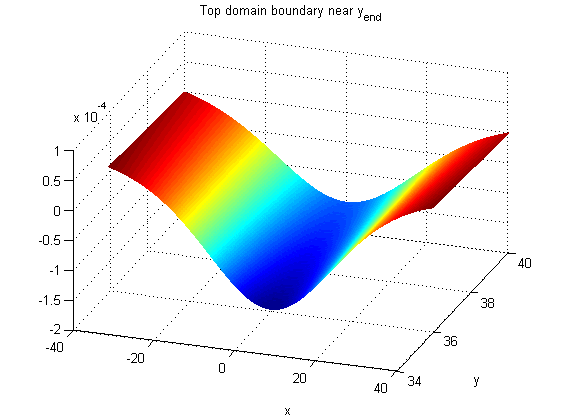
\includegraphics[width=\linewidth]{Pictures/TopBoundary.png}
	\end{minipage}	
	\begin{minipage}[b]{0.45\linewidth}
		
		 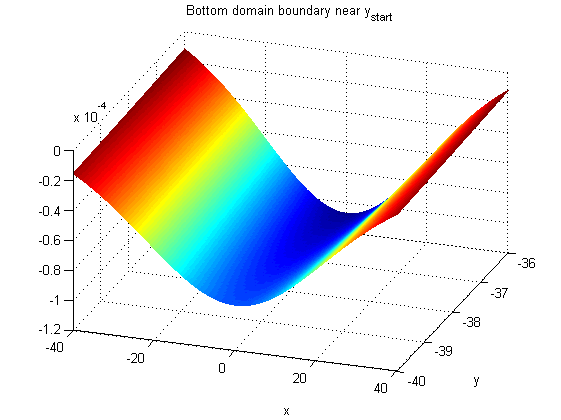
\includegraphics[width=\linewidth]{Pictures/BottomBoundary.png}
	\end{minipage}
	\begin{minipage}[b]{0.45\linewidth}
		
		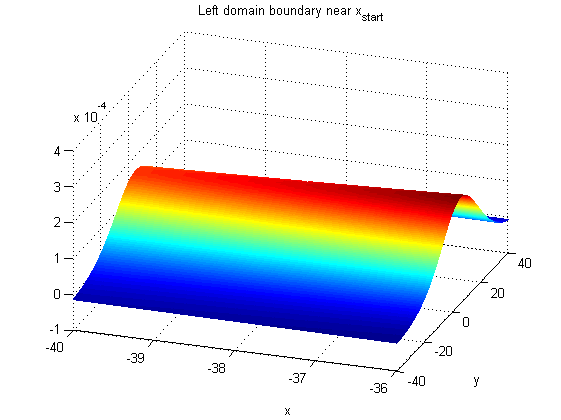
\includegraphics[width=\linewidth]{Pictures/LeftBoundary.png}
	\end{minipage}	
	\begin{minipage}[b]{0.45\linewidth}
		
		 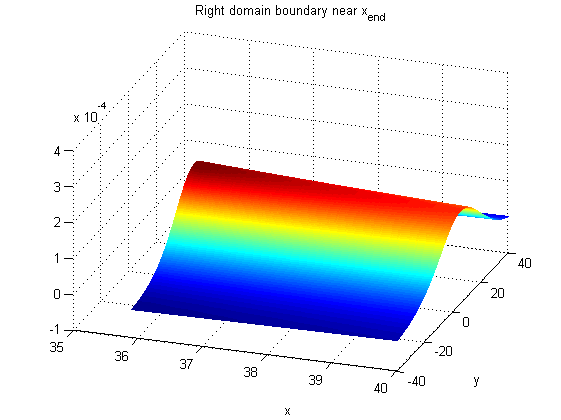
\includegraphics[width=\linewidth]{Pictures/RightBoundary.png}
	\end{minipage}
	\caption{Numerical solution near the boundary for $\beta=3$ and $c = 0.52$}
	\label{fig:boundary}
\end{figure}
\fi
Figure \ref{fig:solMax} displays the evolution of the maximum on the finest grid with the highest approximation order $O(h^6 + \tau^6)$. That is $h=0.05$, $\tau = 0.02$ for the left picture and  $h=0.1$, $\tau = 0.02$ for the right picture. The graph is jagged because the solution maximum is not exactly positioned on the points of the grid $\Omega_h \times T_{\tau}$ but often among them. 

\begin{figure}[!htbp]
	\centering
	\begin{minipage}[b]{0.35\linewidth}
		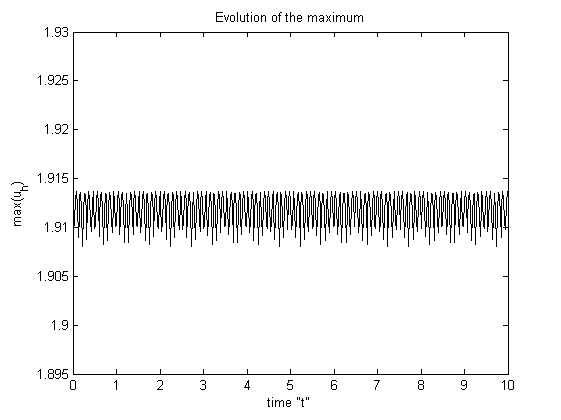
\includegraphics[width=\linewidth]{Pictures/EvolutionOfMaximum_bt3.png}
	\end{minipage}	
	\begin{minipage}[b]{0.35\linewidth}
		 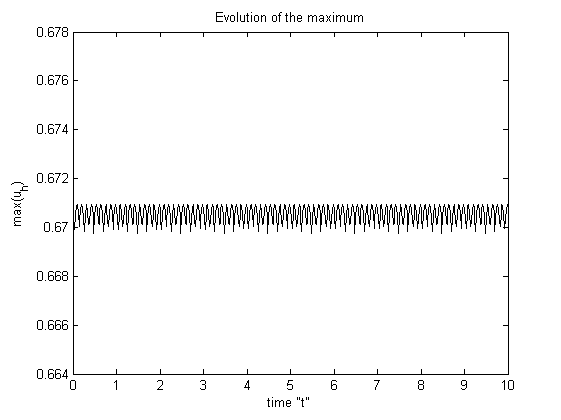
\includegraphics[width=\linewidth]{Pictures/EvolutionOfMaximum_bt1.png}
	\end{minipage}

	\caption{$\beta = 3$, $c=0.52$ on the left panel, and $\beta = 1$, $c=0.9$ on the right panel.}
	\label{fig:solMax}
\end{figure}

The following paragraph is about the complexity of the algorithm viewed from different perspectives. Around 80\% of the computational time goes for the inversion of the discrete operator $A_h = (E - \Delta_h)$. Let us denote with $n_x$, $n_y$ and $n_t$ the point count along $x$, $y$ and $t$ directions on the discrete domain $\Omega_h \times T_{\tau}$, respectively. Then, if $P_A$ denotes the operation count for a single inversion of the $A_h$ operator, the complexity of the algorithm with respect to the space approximation order is given by the following table \rf{tab:b}. \begin{table}[!htbp]
\centering
		\begin{tabular}{||c|c|c|c||}
			\hline
			\hline
      Space approximation order  &        $O(h^2)$    &        $O(h^4)$     &        $O(h^6)$    \\
			\hline 
      Operation count $P_A$ &        $12 * n_y * n_x$    &        $24 * n_y * n_x$     &        $41 * n_y * n_x$    \\
			\hline
			\hline
		\end{tabular}
		\caption{Operations count for a single inversion of the $A_h$ operator.}

\label{tab:b}
\end{table}

The inverse operator $A_h^{-1}$ is a full matrix and working with it requires much more operations $P_A \sim O(n_y^3 * n_x)$. Therefore, it is much cheaper and faster to invert a band matrix with Gauss elimination, e.g. like Thomas algorithm in case of tridiagonal matrix.
Furthermore, the complexity of the algorithm with respect to the time approximation order could be described by the following table \rf{tab:c}. \begin{table}[!htbp]
\centering
		\begin{tabular}{||c|c|c|c||}
			\hline
			\hline
       Time approximation order  &        $O(\tau^2)$    &        $O(\tau^4)$     &        $O(\tau^6)$    \\
			\hline 
      Operation count  &        $P_A$    &        $3 * P_A$     &        $5 * P_A$    \\
			\hline
			\hline
		\end{tabular}
		\caption{Operations count for one TS expansion, where.}

\label{tab:c}
\end{table}

This is because the second order $O(\tau^2)$ requires only one inversion for $D^2 u_h$, the fourth order $O(\tau^4)$ requires three inversions of $A_h$ for the three derivatives $D^2 u_h$, $D^3 u_h$ and $D^4 u_h$ and the sixth order $O(\tau^6)$ requires five inversions of $A_h$ for $D^2 u_h$, $D^3 u_h$, $D^4 u_h$, $D^5 u_h$ and $D^6 u_h$ in the TS expansion.
\begin{figure}[!htbp]
	\centering
	\begin{minipage}[b]{0.31\linewidth}
		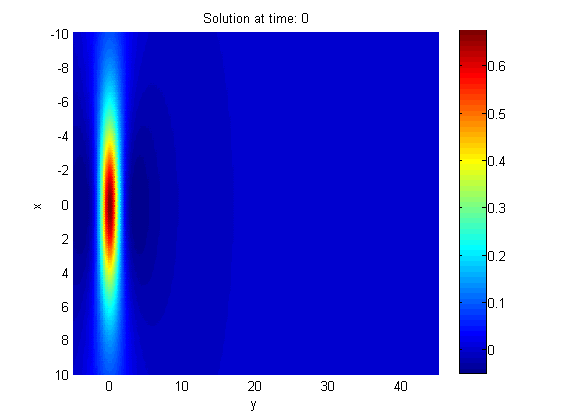
\includegraphics[width=\linewidth]{Pictures/Solution1_t=0.png}
	\end{minipage}	
	\begin{minipage}[b]{0.31\linewidth}
		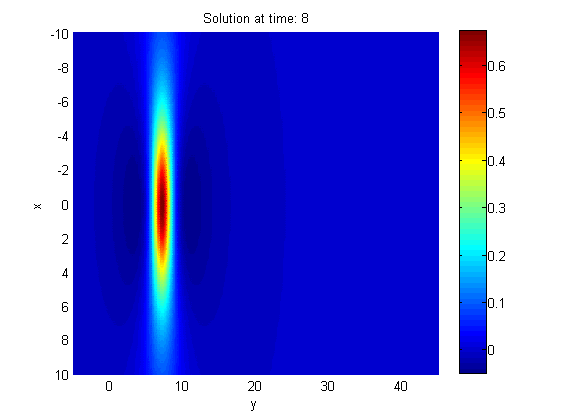
\includegraphics[width=\linewidth]{Pictures/Solution1_t=8.png}
	\end{minipage}	
	\begin{minipage}[b]{0.31\linewidth}
		 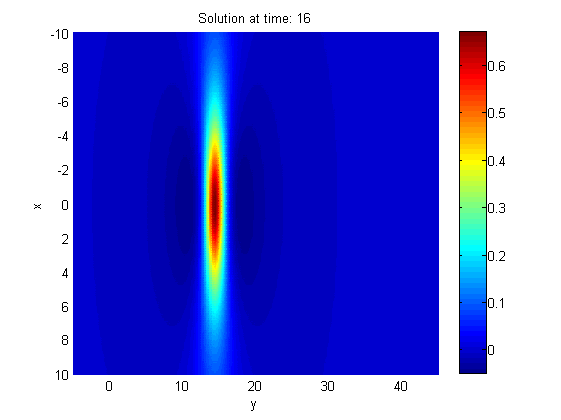
\includegraphics[width=\linewidth]{Pictures/Solution1_t=16.png}
	\end{minipage}
	\begin{minipage}[b]{0.31\linewidth}
		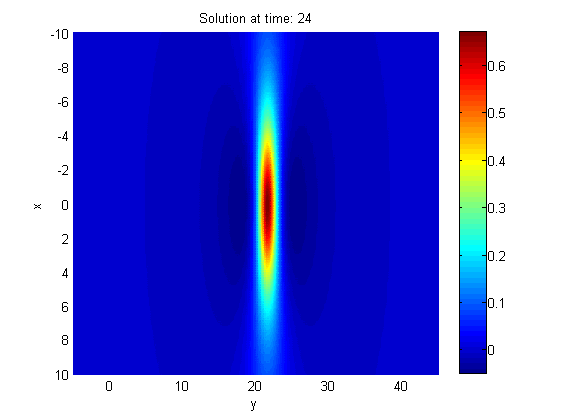
\includegraphics[width=\linewidth]{Pictures/Solution1_t=24.png}
	\end{minipage}	
	\begin{minipage}[b]{0.31\linewidth}
		 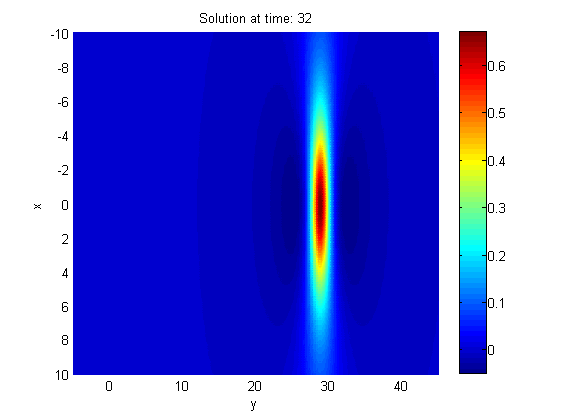
\includegraphics[width=\linewidth]{Pictures/Solution1_t=32.png}
	\end{minipage}
	\begin{minipage}[b]{0.31\linewidth}
		 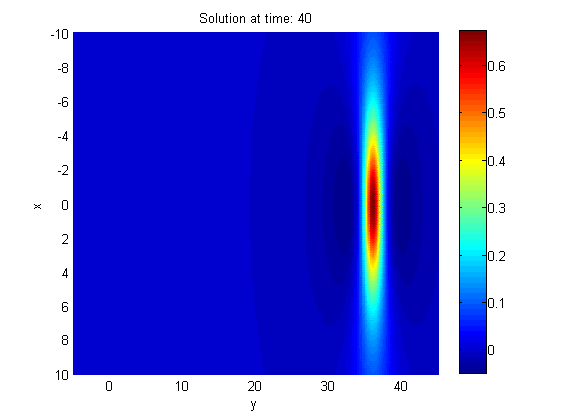
\includegraphics[width=\linewidth]{Pictures/Solution1_t=40.png}
	\end{minipage}
	\caption{Numerical solution of one wave for $\beta=1$ and $c = 0.9$ at times $t=0,8,16,24,32,40$.}
	\label{fig:oneWaveA}
\end{figure}
The complexity of the algorithm is quadratic with respect to the space step length $h$ (the same step is applied along $x$ and $y$ directions) and linear with respect to the time step length $\tau$. Thus, it takes 8 times more time for the algorithm to complete, if $h$ and $\tau$ are two times smaller ($h/2$, $\tau/2$).


Test Wave (see Figure \rf{fig:oneWaveA}). The following test shows single solution wave with $\beta = 1$, $c = 0.9$, $\tau = 0.02$, $h = 0.1$ and $\Omega_h \times T_{\tau}$ $= [40, 40] \times [40, 80] \times [0, 40]$. This is the finest grid for this set with the highest approximation order $O(h^6 + \tau^6)$. Notice that the time domain is increased four times. The wave travels a distance which is $36 = 40*0.9$ units along the $y$ axis.
\begin{figure}[ht]
	\centering
	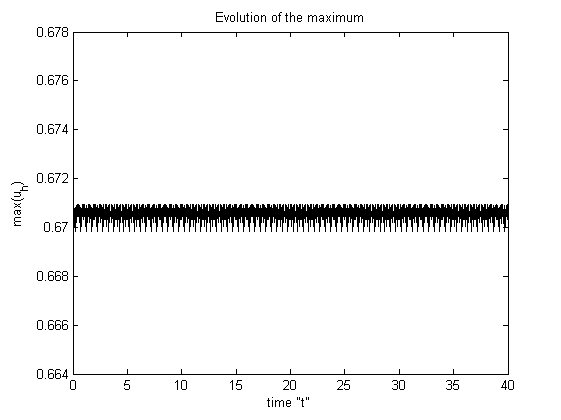
\includegraphics[width=0.4\linewidth]{Pictures/EvolutionOfMaximum.png}

	\caption{Evolution of the maximum for Test Wave.}
	\label{fig:solMax40}
\end{figure}
In order to compare the initial condition $u_h(0)$ with the end solution $u_h(40)$, the last is artificially shifted backwards $y = y^* - 36$ so that both functions are centered with their maximums on $(0,0)$. Thus, it is obtained that $\Vert u_h(40)_{y = y*-36} - u_h(0) \Vert_{L_2} = 0.000812$ and $\Vert u_h(40)_{y = y*-36} - u_h(0) \Vert_{L_\infty} = 0.000039$. The wave behaves like a soliton, i.e. preserves its shape and furthermore figure \ref{fig:solMax40} shows that the solution have stable maximum.
\iffalse
Test 2 (see Figure \rf{fig:oneWaveB}). The following test shows single solution wave with $\beta = 3$, $c = 0.52$, $\tau = 0.02$, $h = 0.1$ and $\Omega_h \times T_{\tau}$ $= [40, 40] \times [40, 80] \times [0, 40]$. The approximation order is $O(h^6 + \tau^6)$ and the time domain is also increased four times compared to results in table \rf{tab:a}. This wave also behave like a soliton, i.e. preserves its shape and maximum even after the collision. Here the wave travels a distance which is $20.8 = 40*0.52$ units along the $y$ axis. It is obtained that $\Vert u_h(40)_{y = y*-20.8} - u_h(0) \Vert_{L_2} = 0.000000$ and $\Vert u_h(40)_{y = y*-20.8} - u_h(0) \Vert_{L_\infty} = 0.000000$.

Figure \ref{fig:solMax40} shows that solutions from both tests have stable maximums.
\begin{figure}[!htbp]
	\centering
	\begin{minipage}[b]{0.4\linewidth}
		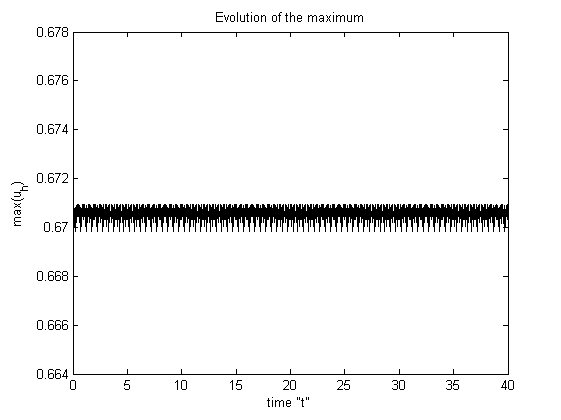
\includegraphics[width=\linewidth]{Pictures/EvolutionOfMaximum.png}
	\end{minipage}	
	\begin{minipage}[b]{0.4\linewidth}
		 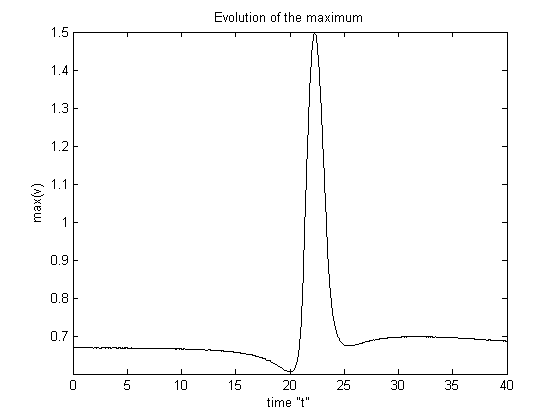
\includegraphics[width=\linewidth]{Pictures/EvolutionOfMaximumTwoWaves.png}
	\end{minipage}

	\caption{Evolution of the maximum for Test 1 (left panel) and Test 2 (right panel).}
	\label{fig:solMax40}
\end{figure}


Test 2 Waves. The following test shows a head-on collision with two solution waves with $\beta = 1$, $c = 0.9$, $\tau = 0.02$, $h = 0.1$ and $\Omega_h \times T_{\tau}$ $= [40, 40] \times [40, 80] \times [0, 40]$. This is the finest grid with the highest approximation order $O(h^6 + \tau^6)$ Waves still behave like a solitons, i.e. preserves its shape and maximum even after the collision.

\begin{figure}[!htbp]
	\centering
	\begin{minipage}[b]{0.31\linewidth}
		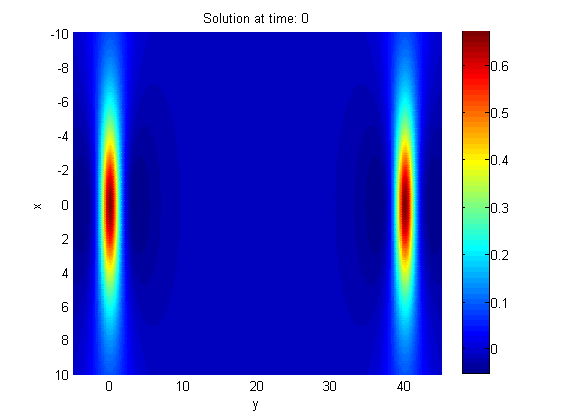
\includegraphics[width=\linewidth]{Pictures/Solution2_t=0.png}
	\end{minipage}	
	\begin{minipage}[b]{0.31\linewidth}
		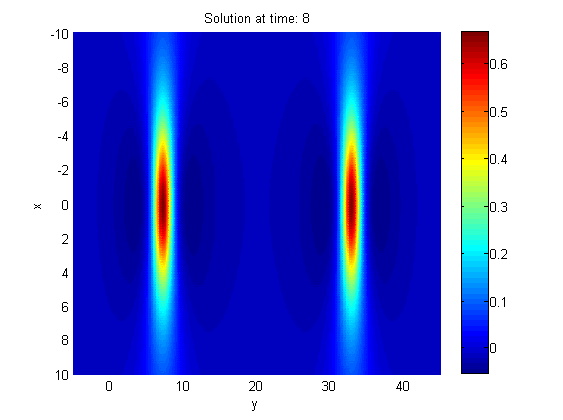
\includegraphics[width=\linewidth]{Pictures/Solution2_t=8.png}
	\end{minipage}	
	\begin{minipage}[b]{0.31\linewidth}
		 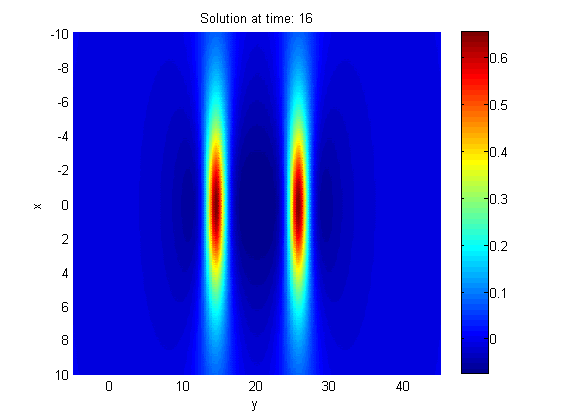
\includegraphics[width=\linewidth]{Pictures/Solution2_t=16.png}
	\end{minipage}
	\begin{minipage}[b]{0.31\linewidth}
		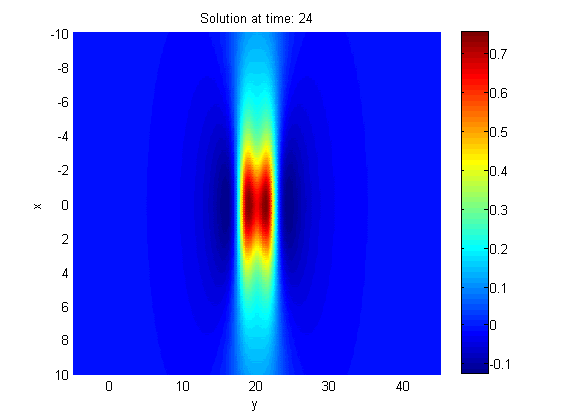
\includegraphics[width=\linewidth]{Pictures/Solution2_t=24.png}
	\end{minipage}	
	\begin{minipage}[b]{0.31\linewidth}
		 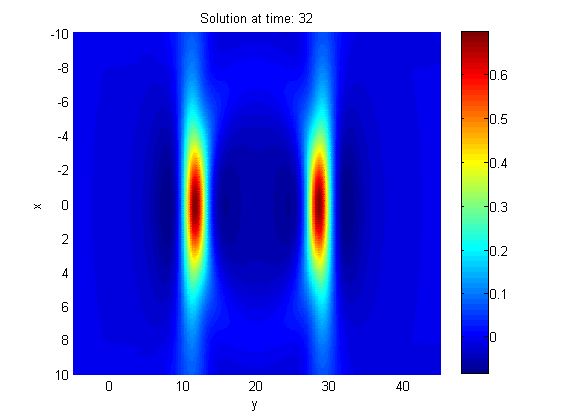
\includegraphics[width=\linewidth]{Pictures/Solution2_t=32.png}
	\end{minipage}
	\begin{minipage}[b]{0.31\linewidth}
		 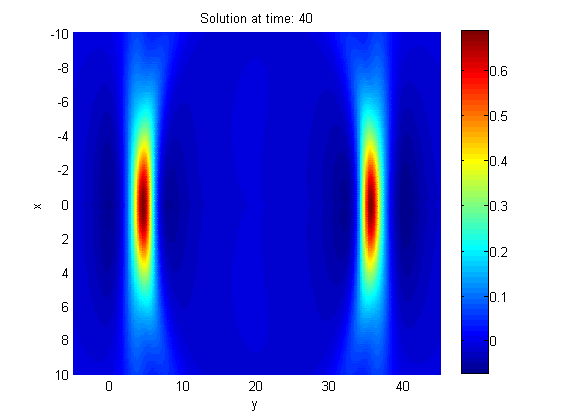
\includegraphics[width=\linewidth]{Pictures/Solution2_t=40.png}
	\end{minipage}
	\caption{Numerical solution of two waves for $\beta=1$ and $c = 0.9$ at times $t=0,8,16,24,32,40$.}
	\label{fig:twoWaves}
\end{figure}

Figure \ref{fig:solMax40} displays the evolution of the solution maximum for Test 1 and Test 2 with one and two waves respectively. In comparison with Figure \ref{fig:solMax}, the time domain is four times bigger with $T_{end}=40$. 
\begin{figure}[!htbp]
	\centering
	\begin{minipage}[b]{0.4\linewidth}
		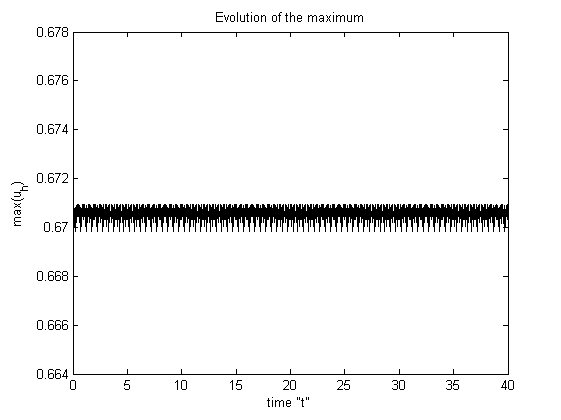
\includegraphics[width=\linewidth]{Pictures/EvolutionOfMaximum.png}
	\end{minipage}	
	\begin{minipage}[b]{0.4\linewidth}
		 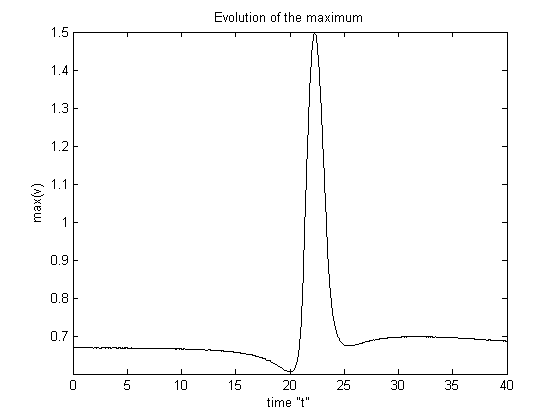
\includegraphics[width=\linewidth]{Pictures/EvolutionOfMaximumTwoWaves.png}
	\end{minipage}

	\caption{Evolution of the maximum for one wave (left panel) and two waves (right panel).}
	\label{fig:solMax40}
\end{figure}
\fi
%=============BEGIN Conclusion========================================
\section{Conclusion}\label{Concl}
%=============BEGIN Conclusion========================================

The investigated solutions are stable and show soliton behavior for wave speeds near the upper limit $c_{max} = 1/\sqrt{\beta}$, $c < c_{max}$, i.e. first, for $c = 0.52$ with $\beta = 3$ and $c_{max} \approx 0.5774$ and second, for  $\beta = 1$, $c=0.9$ and $c_{max} = 1$. The use of regular grid with equidistant step size $h$ turns out to be good choice to test head-on collision of waves. Furthermore, it provides valuable information with sufficient point count on the computational boundary. The performed numerical tests exhibit good convergence and solitonic-like behavior for larger times $t_n \in T_{\tau}$ which validates the TS method. 

%The title of your section
\section{References}

A sample of the references you may find below. Please put your
references in alphabetical order. For abbreviations of names of
journals, use the list:
\URL{http://msc2010.org/MSC2010-CD/extras/serials.pdf}

%The title of your section
\section{Citations}\label{citation}

We use the package \texttt{cite} for creating citations. For citing
use the command \verb@\cite{label}@ or
\verb@\cite[text]{label}@, e.\,g., \cite{BFL},
\cite{Hoff,Whho,Serrin,BFL,BY,A22,quas,Mitt}, or \cite[Chapter
1]{rB}.

%%%%%%%%%%%%%%%%%%%%%%%%%%%%%%%%%%%%%%%%%%%%%%%%%%%%%%%%%%%%%%

%For acknowledgements section, please don't number the section, please begin it with \section*{Acknowledgements.}

\subsection*{Acknowledgments.} We would like to thank you for \textbf{following
the instructions above} very closely in advance. It will definitely
save us lot of time and expedite the process of your paper's
publication.

%%%%%%%%%%%%%%%%%%%%%%%%%%%%%%%%%%%%%%%%%%%%%%%%%%%%%%%%%%%%%%%%

\subsection*{Supports.} The first author is supported by the NSF grant xx-xxxx.

%%%%%%%%%%%%%%%%%%%%%%%%%%%%%%%%%%%%%%%%%%%%%%%%%%%%%%%%%%%%%%%

% References

\begin{thebibliography}{99}

% Example of multiple authors:
\bibitem{BFL}
Y. Benoist, P. Foulon and F. Labourie, % Use `and' connect the last two authors
\emph{Flots d'Anosov a distributions stable et instable differentiables,}
J. Amer. Math. Soc. \textbf{5} (1992), 33--74 (French).

%1
\bibitem{ChChr}
C. Christov, 
\emph{An energy-consistent dispersive shallow-water model}, 
{\it Wave Motion}, \textbf{34} (2001), 161-174.
%8
\bibitem{Ch2011}
C. Christov and J. Choudhury, 
\emph{Perturbation solution  for the 2D Boussinesq equation},       
Mech. Res. Commun., 38 (2011),  274 -- 281.
%6
\bibitem{chr-chr}
M. Christou and C. Christov, 
\emph{Galerkin Spectral Method for the 2D Solitary}
Waves of Boussinesq Paradigm Equation, CP 1186, (2009) 217 -- 225.
%5
\bibitem{chr-chr-07}
M. Christou and C. Christov, 
\emph{Fourier–Galerkin method for 2D solitons of Boussinesq equation}, 
Mathematics and Computers in Simulation, 74, (2007) 82 -- 92.

%2
\bibitem{EllipticProblem}
K. Angelow and N. Kolkovska, 
\emph{Numerical Study of Traveling Wave Solutions to 2D Boussinesq Equation},
Serdica J. Computing,  8, (2018) 3-4.

%7
\bibitem{Ch2012}
C. Christov, 
\emph{Numerical implementation of the asymptotic boundary conditions
for steadily propagating 2D solitons of Boussinesq type equation},       
Math. Computers  Simul., 82 (2012),  1079 -- 1092.

%3
\bibitem{BoundaryProblem}
K. Angelow, 
\emph{New Boundary Condition for the Two Dimensional Stationary Boussinesq Paradigm Equation},
International Journal of Applied Mathematics, (2018).

%9
\bibitem{cher}
A. Chertock, C. Christov and A. Kurganov, 
\emph{Central--upwind schemes for the  Boussinesq paradigm equation},
Comp. Sci. High Performance Comp. IV, NNFM, 113, (2011), 267 -- 281.

\bibitem{dani}
C. Christov, N. Kolkovska and D. Vasileva, 
\emph{On the numerical simulation of unsteady solutions for the 2D Boussinesq paradigm equation},
LNCS, 6046  (2011), 386 -- 394.

\bibitem{critEn}
N. Kolkovska and K. Angelow,
\emph{Numerical computation of the critical energy constant for two-dimensional Boussinesq equations}
AIP Conference Proceedings 1684, 080007 (2015)

\bibitem{Tref}
L.  Trefethen and D. Bau,
\emph{Numerical linear algebra},
1$^{st}$ ed., SIAM, Philadelphia, 1997.

%4
\bibitem{FPS}
T. Lyche,
\emph{Fast Poisson Solvers and FFT}, 
Lecture Notes, University of Oslo, Norway

\bibitem{chd-chr}
J.~Choudhury, C.~Christov, 2D  Solitary waves of  Boussinesq equation, CP75, (2005), 85 -- 90.
 
\bibitem{forn}
B.~Fornberg, 
\emph{Generation of Finite Difference Formulas on Arbitrarily Spaced Grids}, 
Math. Comput., 51(1988),  699 -- 706.

\bibitem{sam}
A.~Samarskii, The theory of difference schemes, M. Dekker,  2001.


\bibitem{A11}
FirstNameInitial.  MiddleNameInitial. LastName, % first name middle initial. and then last name.  Only the first character in the paper title is capitalized.
\emph{Title of the paper,}
Name of the Journal \textbf{Volume} (Year), StaringPage--EndingPage.



% Example of multiple authors:
\bibitem{BFL}
Y. Benoist, P. Foulon and F. Labourie, % Use `and' connect the last two authors
\emph{Flots d'Anosov a distributions stable et instable differentiables,}
J. Amer. Math. Soc. \textbf{5} (1992), 33--74 (French).

% Example of a paper translated in English:
\bibitem{BY}
M.Sh. Birman and D.R. Yafaev,
\emph{The spectral shift function,}  Algebra i Analiz \textbf{4} (1992), No. 5, 1--44 (Russian); Engl. transl.: St. Petersburg Math. J. \textbf{4} (1993), No. 5, 833--870.

% Example of a preprint  with 7 digits archive number:
\bibitem{quas}
M. Entov, L. Polterovich and F. Zapolsky,
\emph{Quasi-morphisms and the Poisson bracket,}
preprint, \arXiv{math/0605406}.

% Example of a thesis:
\bibitem{Hoff}
P. Hoffmann,
\emph{Torsion Cycles and Set Theoretic Complete Intersection},
Ph.D thesis, Washington University in St. Louis, 2006.

\bibitem{Mitt}
F. Mittelbach and M. Goossens, \emph{The LATEX Companion,} 2$^{nd}$ ed., Addison-Wesley Co., Reading,
MA, 2004.

% No author names:
\bibitem{Whho}
\emph{SARS Expert Committee, SARS in Hong Kong: From Experience to
Action}, Report of Hong Kong SARS Expert Committee,
2003. Available from: \URL{http://www.sars-expertcom.gov.hk/english/reports/reports.html}.


% Example of a paper in Academic Press or a book:
\bibitem{Serrin}
J. Serrin,
\emph{Gradient estimates for solutions of nonlinear elliptic and parabolic equations,}
Contributions to Nonlinear Functional Analysis (eds. E.H. Zarantonello and Author 2), Academic Press, 1971, 33--75.

% Example of a book in the reference:
\bibitem{rB}
J.  Smoller,
\emph{Shock Waves and Reaction-Diffusion Equations},
2$^{nd}$ ed.,  Springer-Verlag, New York, 1994.

% Example of a preprint  with 8 digits archive number:
\bibitem{Te2008}
A. Teplinsky,
\emph{Herman's theory revisited,} preprint,
\arXiv{0707.0078}.

%
\bibitem{A22}
C.  Wolf,
\emph{A mathematical model for the propagation of a hantavirus in structured populations,}
Discrete Contin. Dyn. Syst. Ser. B \textbf{4} (2004), 1065--1089.



\end{thebibliography}


%%%%%%%%%%%%%%%%%%%%%%%%%%%%%%

\EndPaper%%%%  do not remove this command

%%%%%%%%%%%%%%%%%%%%%%%%%%%%%%%%%%%%%%%%%%%%%%%%%%%%%%%

\end{document}
